\chapter{Resultados}
  \section{Estadísticas del MicroMundo}
    Todos las estadísticas fueron ejecutadas considerando el mismo mundo(mapa) y la misma cantidad de generaciones (1000). El único factor que cambia es la cantidad de especies distribuidas de forma uniforme sobre el mapa. Los resultados se muestran a continuación.
    \subsection{MicroMundo al 1\%}      
      \begin{figure}[h!]
        \centering
          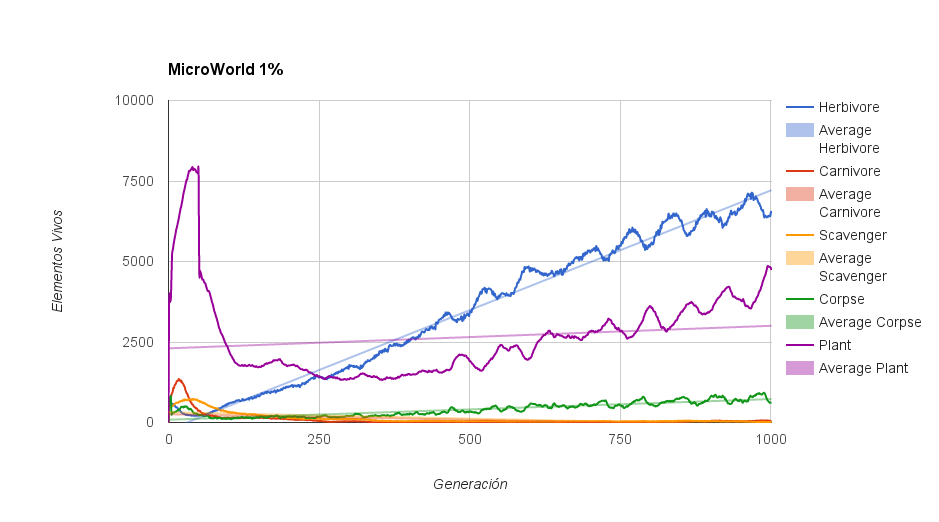
\includegraphics[width=\textwidth]{./images/0_01.png}
          \caption{Resultados del MicroMundo al 1\% de distribución.} 
      \end{figure}      
      Como puede verse, existe un punto donde el mundo se llena de plantas, entre la generación 0 y la 100, conforme pasan las generaciones, gracias a la gran existencia de alimento, los herbívoros empiezan a dominar en cuanto elementos vivos. Durante las primeras generaciones los carnívoros se visualizan como la especie dominante, sin embargo, al llegar punto donde la vegetación alcanza su máximo, el declive de éstos comienza, llegando a valores mínimos pero sin extinguirse.
    \subsection{MicroMundo al 5\%}      
      \begin{figure}[h!]
        \centering
          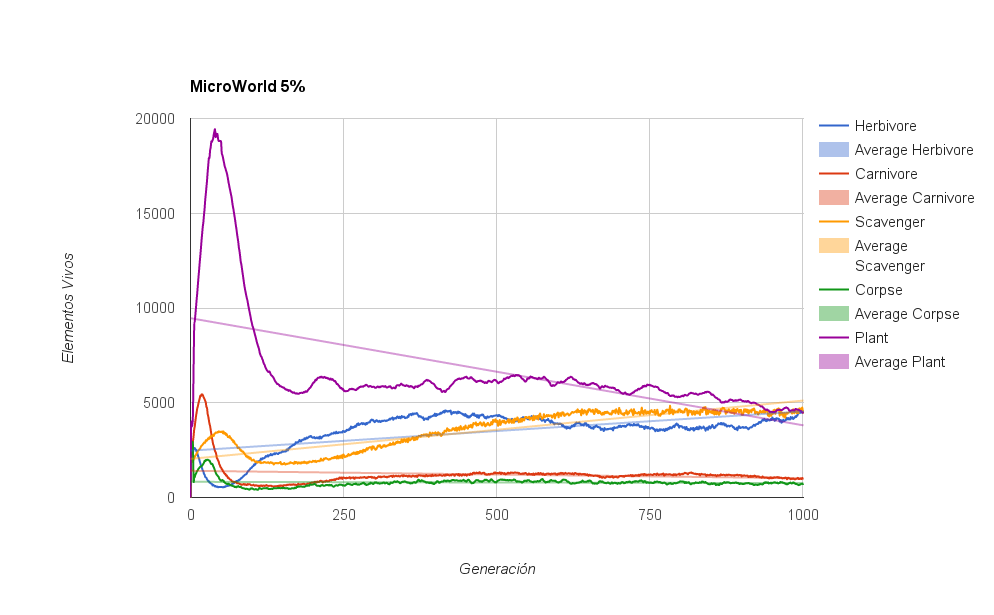
\includegraphics[width=\textwidth]{./images/0_05.png}
          \caption{Resultados del MicroMundo al 5\% de distribución.} 
      \end{figure}      
      Tomando ahora las estadísticas de los animales al 5\%, se puede ver que el comportamiento es semejante durante las primeras generaciones, sin embargo, conforme pasan las generaciones las Plantas, Herbívoros y Carroñeros parecen estabilizarse. 
      
      Los carnívoros y cadáveres se mantienen constantes pero sin crecimiento alguno, esto podría ser visualizado considerando que éstos pueden encontrarse lejos de fuentes de agua y eso propicia su poco crecimiento. Los carnívoros se mantienen de aquellos animales que se alejan de los cuerpos de agua, y éstos últimos a su vez generan los cadáveres que mantienen dicho equilibrio.
    \linebreak
    \newpage
    \subsection{MicroMundo al 10\%}      
      \begin{figure}[h!]
        \centering
          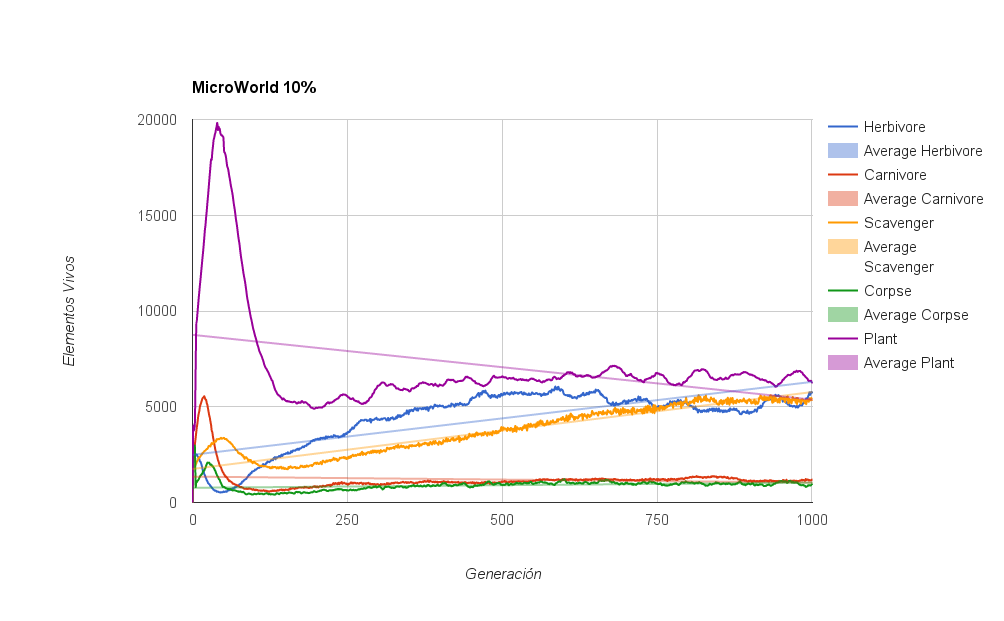
\includegraphics[width=\textwidth]{./images/0_1.png}
          \caption{Resultados del MicroMundo al 10\% de distribución.} 
      \end{figure}      
      Tomando ahora las estadísticas de los animales al 10\%, se muestra nuevamente que el comportamiento es muy semejante a la distribución del 5\%, pero ésta muestra una mayor tendencia a la estabilidad entre Herbívoros, Plantas y Carroñeros desde la generación 500, dando a entender que los factores iniciales (distribución de la vegetación y agua en el mundo inicial) influye pero sólo disminuye el número de generaciones para que se logren puntos críticos de cruce entre las especies. El caso de los Carnívoros y cadáveres sigue siendo semejante.
    \linebreak
    \newpage
    \subsection{MicroMundo al 50\%}      
      \begin{figure}[h!]
        \centering
          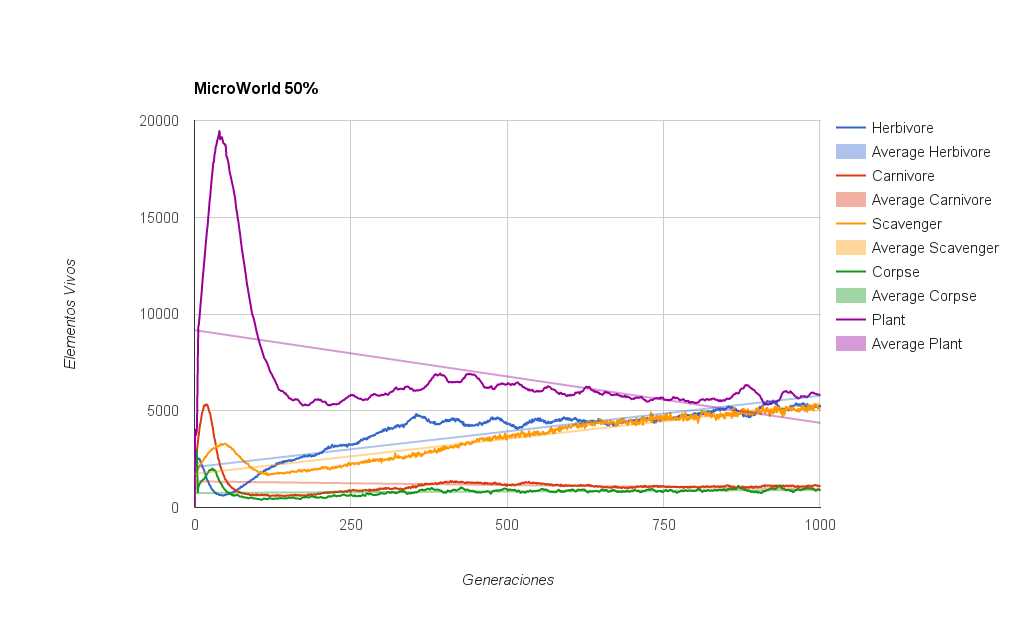
\includegraphics[width=\textwidth]{./images/0_5.png}
          \caption{Resultados del MicroMundo al 50\% de distribución.} 
      \end{figure}      
      Finalmente las estadísticas de los animales al 50\%, el comportamiento de los animales vivos dentro del mundo generado es muy semejante durante las cuatro simulaciones; ésta nos muestra una estabilidad más definida entre los Herbívoros y Carroñeros a partir de la generación 500, donde ambas curvas son muy semejantes. 

      Posteriormente se unen las plantas como elemento estable casi después de la generación 750. 

      El caso de los carnívoros y cadáveres no presenta un cambio drástico, se mantienen estables después de la generación 50 (aproximadamente), sin embargo, nunca se extinguen.
    \linebreak
    \newpage
    \subsection{MicroMundo modificado (Considerando valores previos)}
      Se procedió a la simulación de un nuevo micromundo, tomando los mismos parámetros de entrada pero modificando el comportamiento de los carnívoros (aumentando su rango de visión) y disminuyendo los puntos de vida de las plantas, obteniendo los resultados mostrados en la gráfica; además de tomar una distribución al 15\% (Promedio del porcentaje de todas las distribuciones).
      \begin{figure}[h!]
        \centering
          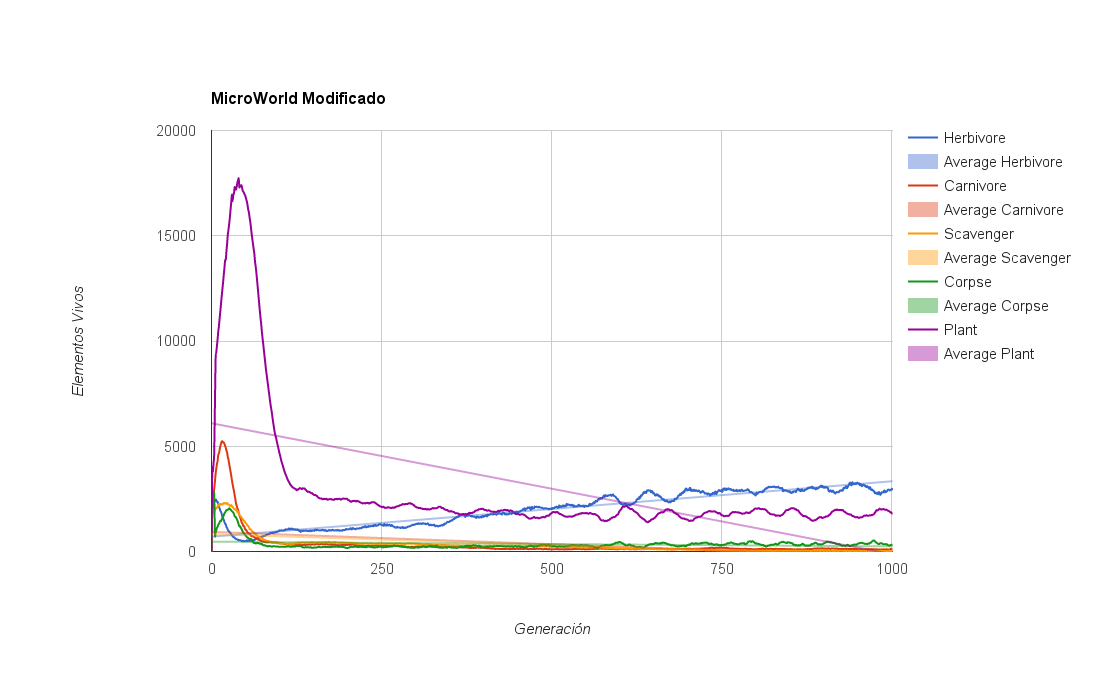
\includegraphics[width=\textwidth]{./images/Modified.png}
          \caption{Resultados del MicroMundo al 15\% de distribución, Acciones modificadas.} 
      \end{figure} 
      \linebreak

      La gráfica nos muestra un comportamiento semejante (gracias a los valores de entrada del mapa) y la distribución uniforme usada, sin embargo, también nos permite la visualización de cómo se estabilizan los animales carnívoros, carroñeros y la cantidad de cadáveres desde la generación 500. A pesar de obtener una nueva estabilidad, los herbívoros se encuentran oscilando con los valores de la vegetación desde la generación 300, subiendo y bajando pero sin llegar a tener una gran diferencia.

      El mapa de entrada es un factor muy importante, ya que define por mucho en todas las pruebas las primeras 100 generaciones de una forma muy semejante. La cantidad de agua, arbustos y agua propicia el crecimiento o decaimiento de ciertas especies.